%iffalse
\let\negmedspace\undefined
\let\negthickspace\undefined
\documentclass[journal,12pt,onecolumn]{IEEEtran}
\usepackage{cite}
\usepackage{amsmath,amssymb,amsfonts,amsthm}
\usepackage{algorithmic}
\usepackage{graphicx}
\usepackage{textcomp}
\usepackage{xcolor}
\usepackage{txfonts}
\usepackage{listings}
\usepackage{enumitem}
\usepackage{enumitem,multicol}
\usepackage{mathtools}
\usepackage{gensymb}
\usepackage{comment}
\usepackage[breaklinks=true]{hyperref}
\usepackage{tkz-euclide} 
\usepackage{listings}
\usepackage{gvv}                                        
%\def\inputGnumericTable{}                                 
\usepackage[latin1]{inputenc}                                
\usepackage{color}                                            
\usepackage{array}                                            
\usepackage{longtable}                                       
\usepackage{calc}                                             
\usepackage{multirow}                                         
\usepackage{hhline}                                           
\usepackage{ifthen}                                           
\usepackage{lscape}
\usepackage{tabularx}
\usepackage{array}
\usepackage{float}
\usepackage[american,siunitx]{circuitikz}
\usetikzlibrary{arrows,shapes,calc,positioning}
\usepackage{pgfplots}


\newtheorem{theorem}{Theorem}[section]
\newtheorem{problem}{Problem}
\newtheorem{proposition}{Proposition}[section]
\newtheorem{lemma}{Lemma}[section]
\newtheorem{corollary}[theorem]{Corollary}
\newtheorem{example}{Example}[section]
\newtheorem{definition}[problem]{Definition}
\newcommand{\BEQA}{\begin{eqnarray}}
\newcommand{\EEQA}{\end{eqnarray}}
\newcommand{\define}{\stackrel{\triangle}{=}}
\theoremstyle{remark}
\newtheorem{rem}{Remark}
\pgfplotsset{compat=1.18}

% Marks the beginning of the document
\begin{document}
\bibliographystyle{IEEEtran}
\vspace{3cm}

\title{ME-2021}
\author{EE24Btech11022 - Eshan Sharma}
\maketitle

\renewcommand{\thefigure}{\theenumi}
\renewcommand{\thetable}{\theenumi}



\begin{enumerate}
\item Consider a two degree of freedom system as shown in the figure, where $PQ$ is a rigid uniform rod of length $b$ and mass $m$.\\

\begin{center}
	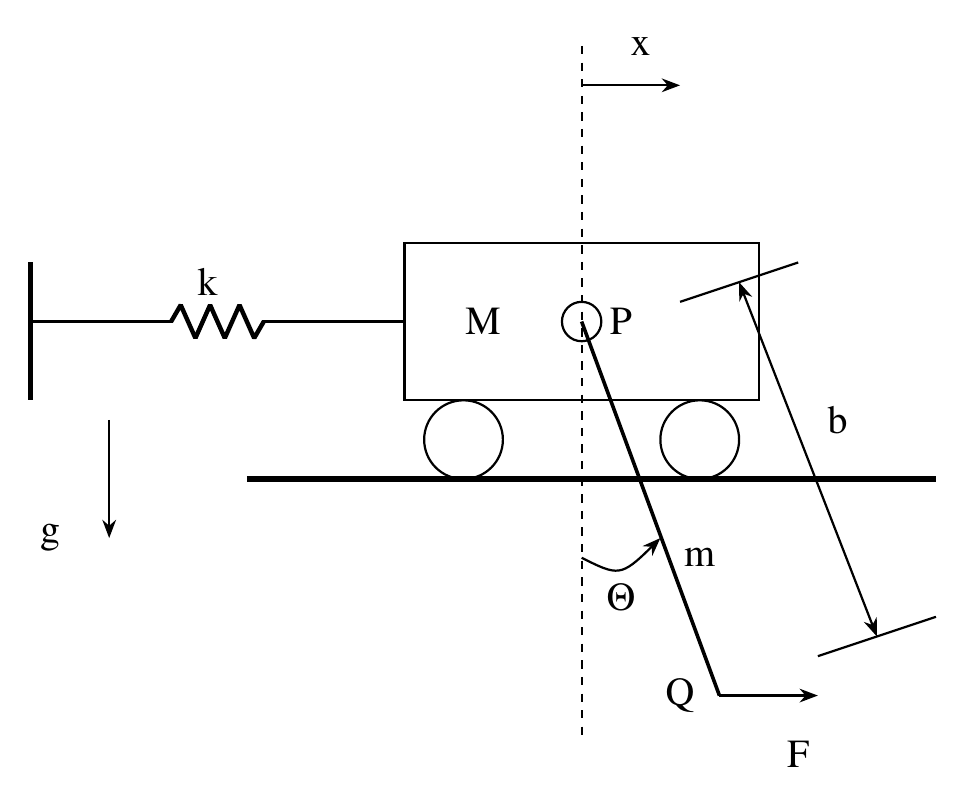
\begin{tikzpicture}
		\draw [line width=2pt, short] (8,11.25) -- (16.75,11.25);
		\draw [line width=2pt, short] (5.25,14) -- (5.25,12.25);
		\draw [line width=0.8pt, dashed] (12.25,16.75) -- (12.25,8);
		\draw [ line width=0.8pt ] (10,14.25) rectangle (14.5,12.25);
		\draw [ line width=0.8pt ] (10.75,11.75) circle (0.5cm);
		\draw [ line width=0.8pt ] (13.75,11.75) circle (0.5cm);
		\draw [ line width=0.8pt](5.25,13.25) to[R] (10,13.25);
		\draw [line width=0.8pt, ->, >=Stealth] (12.25,16.25) -- (13.5,16.25);
		\draw [line width=0.8pt, ->, >=Stealth] (6.25,12) -- (6.25,10.5);
		\draw [line width=1.3pt, short] (12.25,13.25) -- (14,8.5);
		\draw [line width=0.8pt, short] (15.25,9) -- (16.75,9.5);
		\draw [line width=0.8pt, short] (13.5,13.5) -- (15,14);
		\draw [line width=0.8pt, <->, >=Stealth] (14.25,13.75) -- (16,9.25);
		\draw [line width=0.8pt, ->, >=Stealth] (14,8.5) -- (15.25,8.5);
		\draw [line width=0.8pt, ->, >=Stealth] (12.25,10.25) .. controls (12.75,10) and (12.75,10) .. (13.25,10.5) ;
		\node [font=\Large] at (5.5,10.5) {g};
		\node [font=\Large] at (7.5,13.75) {k};
		\node [font=\Large] at (13,16.75) {x};
		\node [font=\Large] at (11,13.25) {M};
		\node [font=\Large] at (12.75,13.25) {P};
		\node [font=\Large] at (13.75,10.25) {m};
		\node [font=\Large] at (12.75,9.75) {$\Theta$};
		\node [font=\Large] at (15.5,12) {b};
		\node [font=\Large] at (15,7.75) {F};
		\draw [ line width=0.8pt ] (12.25,13.25) circle (0.25cm);
		\node [font=\Large] at (13.5,8.5) {Q};
	\end{tikzpicture}
	
\end{center}
Assume that the spring deflects only horizontally and force $F$ is applied horizontally at $Q$. For this system, the Lagrangian $L$ is:


\begin{enumerate}
	\item $ \frac{1}{2}(M + m)\dot{x}^2 + \frac{1}{6}mb^2\dot{\theta}^2 - \frac{1}{2}kx^2 + mg \frac{b}{2}\cos\theta $\\
	\item $ \frac{1}{2}(M + m)\dot{x}^2 + \frac{1}{2}mb\dot{\theta}\dot{x} \cos \theta + \frac{1}{6}mb^2\dot{\theta}^2 - \frac{1}{2}kx^2 + mg \frac{b}{2}\cos\theta $\\
	\item $ \frac{1}{2}M\dot{x}^2 + \frac{1}{2}mb\dot{\theta}\dot{x} \cos \theta + \frac{1}{6}mb^2\dot{\theta}^2 - \frac{1}{2}kx^2 $\\
	\item $ \frac{1}{2}M\dot{x}^2 + \frac{1}{2}mb\dot{\theta}\dot{x} \cos \theta + \frac{1}{6}mb^2\dot{\theta}^2 - \frac{1}{2}kx^2 + mg \frac{b}{2} \cos \theta + Fb \sin \theta $
\end{enumerate}

	
\item A right solid circular cone standing on its base on a horizontal surface is of height $H$ and base radius $R$. The cone is made of a material with specific weight $w$ and elastic modulus $E$. The vertical deflection at the mid-height of the cone due to self-weight is given by
\begin{enumerate}
	\item $\frac{wH^{2}}{8E}$
	\item $\frac{wH^{2}}{6E}$
	\item $\frac{wRH}{8E}$
	\item $\frac{wRH}{6E}$
\end{enumerate}

\item A tappet valve mechanism in an $IC$ engine comprises a rocker arm $ABC$ that is hinged at $B$ as shown in the figure. The rocket is assumed rigid and it oscillates about the hinge $B$. The mass moment of inertia of the rocker about $B$ is $10^{-4} kg.m^{2}$. The rocker arm dimensions are $a = 3.5cm$ and $b=2.5cm$. A pushrod pushes the rocker at location $A$, when moved vertically by a cam that rotates at $N$ rpm. The pushrod is assumed massless and has a stiffness of $15 N/mm$. At the other end $C$, the rocker pushes a valve against a spring of stiffness $10 N/mm$. The valve is assumed massless and rigid.\\
\begin{center}
	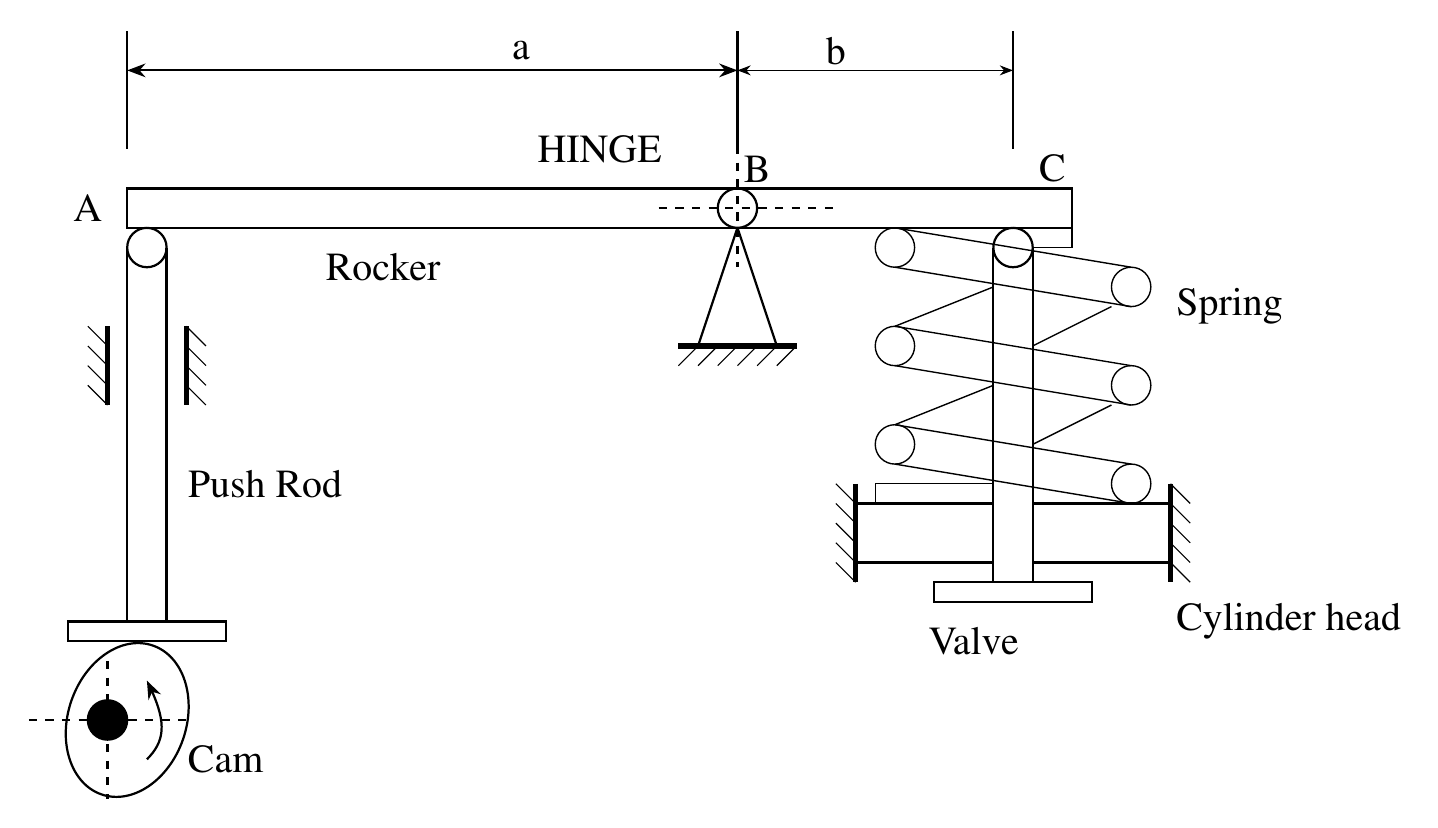
\begin{tikzpicture}
		\draw [ line width=0.8pt ] (6.75,13.75) rectangle (18.75,13.25);
		\draw [line width=0.8pt, short] (14.5,13.25) -- (14,11.75);
		\draw [line width=0.8pt, short] (14.5,13.25) -- (15,11.75);
		\draw [line width=0.8pt, short] (14,11.75) -- (15,11.75);
		\draw [ line width=0.8pt ] (14.5,13.5) circle (0.25cm);
		\draw [ line width=0.8pt ] (7,13) circle (0.25cm);
		\draw [line width=0.8pt, short] (6.75,13) -- (6.75,8.75);
		\draw [line width=0.8pt, short] (7.25,13) -- (7.25,8.75);
		\draw [ line width=0.8pt ] (6,8.25) rectangle (8,8);
		\draw [ line width=0.8pt , rotate around={-19:(6.75,7)}] (6.75,7) ellipse (0.75cm and 1cm);
		\draw [ fill={rgb,255:red,0; green,0; blue,0} , line width=0.8pt ] (6.5,7) circle (0.25cm);
		\draw [line width=0.8pt, dashed] (6.5,7.75) -- (6.5,6);
		\draw [line width=0.8pt, dashed] (5.5,7) -- (7.5,7);
		\draw [line width=0.8pt, ->, >=Stealth] (7,6.5) .. controls (7.25,6.75) and (7.25,7) .. (7,7.5) ;
		\draw [ line width=0.8pt ] (18,13) circle (0.25cm);
		\draw [line width=0.8pt, short] (17.75,13) -- (17.75,10.75);
		\draw [line width=0.8pt, short] (18.25,13) -- (18.25,10.75);
		\draw [ line width=0.8pt ] (17,8.75) rectangle (19,8.5);
		\draw [line width=2pt, short] (16,10) -- (16,8.75);
		\draw [line width=2pt, short] (20,10) -- (20,8.75);
		\draw [line width=2pt, short] (13.75,11.75) -- (15.25,11.75);
		\draw [line width=2pt, short] (6.5,12) -- (6.5,11);
		\draw [line width=2pt, short] (7.5,12) -- (7.5,11);
		\draw [line width=0.8pt, short] (6.75,15.75) -- (6.75,14.25);
		\draw [line width=0.8pt, short] (14.5,15.75) -- (14.5,14.25);
		\draw [line width=0.8pt, short] (18,15.75) -- (18,14.25);
		\draw [line width=0.8pt, <->, >=Stealth] (6.75,15.25) -- (14.5,15.25);
		\draw [line width=0.8pt, dashed] (14.5,14.5) -- (14.5,12.75);
		\draw [line width=0.8pt, dashed] (13.5,13.5) -- (15.75,13.5);
		\draw [<->, >=Stealth] (14.5,15.25) -- (18,15.25);
		\draw [line width=0.8pt, short] (17.75,10.75) -- (17.75,10.5);
		\draw [line width=0.8pt, short] (18.25,10.75) -- (18.25,10.5);
		\draw [line width=0.8pt, short] (6.75,8.75) -- (6.75,8.25);
		\draw [line width=0.8pt, short] (7.25,8.75) -- (7.25,8.25);
		\draw [line width=0.8pt, short] (17.75,10.5) -- (17.75,8.75);
		\draw [line width=0.8pt, short] (18.25,10.5) -- (18.25,8.75);
		\draw [ line width=0.5pt ] (16.5,13) circle (0.25cm);
		\draw [ line width=0.5pt ] (19.5,12.5) circle (0.25cm);
		\draw [ line width=0.5pt ] (16.5,11.75) circle (0.25cm);
		\draw [ line width=0.5pt ] (19.5,11.25) circle (0.25cm);
		\draw [ line width=0.5pt ] (16.5,10.5) circle (0.25cm);
		\draw [ line width=0.5pt ] (19.5,10) circle (0.25cm);
		\draw [line width=0.8pt, short] (18.25,9.75) -- (20,9.75);
		\draw [line width=0.8pt, short] (18.25,9) -- (20,9);
		\draw [line width=0.8pt, short] (17.75,9.75) -- (16,9.75);
		\draw [line width=0.8pt, short] (17.75,9) -- (16,9);
		\draw [line width=0.5pt, short] (16.5,13.25) -- (19.5,12.75);
		\draw [line width=0.5pt, short] (16.5,12.75) -- (19.5,12.25);
		\draw [line width=0.5pt, short] (16.5,12) -- (19.5,11.5);
		\draw [line width=0.5pt, short] (16.5,11.5) -- (19.5,11);
		\draw [line width=0.5pt, short] (16.5,10.75) -- (19.5,10.25);
		\draw [line width=0.5pt, short] (16.5,10.25) -- (19.5,9.75);
		\draw [line width=0.5pt, short] (18.25,13) -- (18.75,13);
		\draw [line width=0.5pt, short] (18.75,13.25) -- (18.75,13);
		\draw [line width=0.5pt, short] (16.5,12) -- (17.75,12.5);
		\draw [line width=0.5pt, short] (18.25,11.75) -- (19.25,12.25);
		\draw [line width=0.5pt, short] (16.5,10.75) -- (17.75,11.25);
		\draw [line width=0.5pt, short] (17.75,10) -- (16.25,10);
		\draw [line width=0.5pt, short] (16.25,10) -- (16.25,9.75);
		\draw [line width=0.5pt, short] (18.25,10.5) -- (19.25,11);
		\draw [short] (6.25,12) -- (6.5,11.75);
		\draw [short] (6.25,11.75) -- (6.5,11.5);
		\draw [short] (6.25,11.5) -- (6.5,11.25);
		\draw [short] (6.25,11.25) -- (6.5,11);
		\draw [short] (7.5,12) -- (7.75,11.75);
		\draw [short] (7.5,11.75) -- (7.75,11.5);
		\draw [short] (7.5,11.5) -- (7.75,11.25);
		\draw [short] (7.5,11.25) -- (7.75,11);
		\draw [short] (14,11.75) -- (13.75,11.5);
		\draw [short] (14.25,11.75) -- (14,11.5);
		\draw [short] (14.5,11.75) -- (14.25,11.5);
		\draw [short] (14.75,11.75) -- (14.5,11.5);
		\draw [short] (15,11.75) -- (14.75,11.5);
		\draw [short] (15.25,11.75) -- (15,11.5);
		\draw [short] (15.75,10) -- (16,9.75);
		\draw [short] (15.75,9.75) -- (16,9.5);
		\draw [short] (15.75,9.5) -- (16,9.25);
		\draw [short] (15.75,9.25) -- (16,9);
		\draw [short] (15.75,9) -- (16,8.75);
		\draw [short] (20,10) -- (20.25,9.75);
		\draw [short] (20,9.75) -- (20.25,9.5);
		\draw [short] (20,9.5) -- (20.25,9.25);
		\draw [short] (20,9.25) -- (20.25,9);
		\draw [short] (20,9) -- (20.25,8.75);
		\node [font=\Large] at (8,6.5) {Cam};
		\node [font=\Large] at (8.5,10) {Push Rod};
		\node [font=\Large] at (10,12.75) {Rocker};
		\node [font=\Large] at (12.75,14.25) {HINGE};
		\node [font=\Large] at (20.75,12.25) {Spring};
		\node [font=\Large] at (17.5,8) {Valve};
		\node [font=\Large] at (21.5,8.25) {Cylinder head};
		\node [font=\Large] at (11.75,15.5) {a};
		\node [font=\Large] at (15.75,15.5) {b};
		\node [font=\Large] at (6.25,13.5) {A};
		\node [font=\Large] at (14.75,14) {B};
		\node [font=\Large] at (18.5,14) {C};
	\end{tikzpicture}
	
\end{center}
Resonance in the rocker system occurs when the cam shaft runs at a speed of \_\_\_\_\_\_\_\_\_ rpm(round off to two decimal places).
\begin{enumerate}
	\item $496$
	\item $4739$
	\item $790$
	\item $2369$
\end{enumerate}

\item Customers arrive at a shop according to the Poisson distribution with a mean of 10 customers/hour. The manager notes that no customer arrives for the first 3 minutes after the shop opens. The probability that a customer arrives within the next 3 minutes is
\begin{enumerate}
	\item 0.39
	\item 0.86
	\item 0.50
	\item 0.61
\end{enumerate}
	
\item Let $f(x) = x^2 - 2x + 2$ be a continuous function defined on $x \in [1, 3]$. The point $x$ at which the tangent of $f(x)$ becomes parallel to the straight line joining $f(1)$ and $f(3)$ is
\begin{enumerate}
	\item 0
	\item 1
	\item 2
	\item 3
\end{enumerate}

\item Activities $A$, $B$, $C$, and $D$ form the critical path for a project with a PERT network. The means and variances of the activity duration for each activity are given below. All activity durations follow the Gaussian (normal) distribution and are independent of each other.

\begin{table}[ht!]
	\centering
	\resizebox{0.5\textwidth}{!}{
		\begin{tabular}[12pt]{ |c|c|c|}
    \hline
    \textbf{Symbol} & \textbf{Value} & \textbf{Description} \\
    \hline
    \textbf{S} & $3cm$ & length of side of square\\
    \hline
    \end{tabular}

	}
\end{table}

The probability that the project will be completed within 40 days is \_\_\_\_\_\_\_\_\_\_ (round off to two decimal places).

(Note: Probability is a number between 0 and 1).\\

\item A true centrifugal casting operation needs to be performed horizontally to make copper tube sections with an outer diameter of 250 mm and an inner diameter of 230 mm. The value of acceleration due to gravity, $g = 10$ m/s$^2$. If a $G$-factor (ratio of centrifugal force to weight) of 60 is used for casting the tube, the rotational speed required is \_\_\_\_\_\_\_\_\_\_ rpm (round off to the nearest integer).\\

\item The resistance spot welding of two 1.55 mm thick metal sheets is performed using a welding current of 10000 A for 0.25 s. The contact resistance at the interface of the metal sheets is 0.0001 $\Omega$. The volume of weld nugget formed after welding is 70 mm$^3$. Considering the heat required to melt a unit volume of metal is 12 J/mm$^3$, the thermal efficiency of the welding process is \_\_\_\_\_\_\_\_\_\_\% (round off to one decimal place). \\

\item An orthogonal cutting operation is performed using a single-point cutting tool with a rake angle of $12^\circ$ on a lathe. During turning, the cutting force and the friction force are 1000 N and 600 N, respectively. If the chip thickness and the uncut chip thickness during turning are 1.5 mm and 0.75 mm, respectively, then the shear force is \_\_\_\_\_\_\_\_\_\_ N (round off to two decimal places).\\

\item In a grinding operation of a metal, specific energy consumption is 15 $ \text{J/mm}^3 $. If a grinding wheel with a diameter of 200 mm is rotating at 3000 rpm to obtain a material removal rate of 6000 $ \text{mm}^3/\text{min} $, then the tangential force on the wheel is \_\_\_\_\_\_\_\_\_\_N (round off to two decimal places).\\

\item A 200 mm wide plate having a thickness of 20 mm is fed through a rolling mill with two rolls. The radius of each roll is 300 mm. The plate thickness is to be reduced to 18 mm in one pass using a roll speed of 50 rpm. The strength coefficient $ K $ of the work material flow curve is 300 MPa and the strain hardening exponent, $ n $ is 0.2. The coefficient of friction between the rolls and the plate is 0.1. If the friction is sufficient to permit the rolling operation, then the roll force will be \_\_\_\_\_\_\_\_\_\_kN (round off to the nearest integer).\\

\item The $ XY $ table of a NC machine tool is to move from $ P(1,1) $ to $ Q(51,1) $; all coordinates are in mm. The pitch of the NC drive leadscrew is 1 mm. If the backlash between the leadscrew and the nut is 1.8$ ^\circ $, then the total backlash of the table on moving from $ P $ to $ Q $ is \_\_\_\_\_\_\_\_\_\_ mm (round off to two decimal places).\\

\item Consider a single machine workstation to which jobs arrive according to a Poisson distribution with a mean arrival rate of 12 jobs/hour. The process time of the workstation is exponentially distributed with a mean of 4 minutes. The expected number of jobs at the workstation at any given point of time is \_\_\_\_\_\_\_\_\_\_ (round off to the nearest integer).


\end{enumerate}
\end{document}


